\section{Polygonal Action in Chain Drives}

The speed of a chain\marginnote{Abstract \citep{mahalingam1958}} is subject to periodic fluctuations, even for a constant speed of the driving sprocket, due to the fact that a chain lying on a sprocket forms a polygon rather than a circle. It is shown that the dynamic loading of the chain due to this ``polygonal action'' is similar to that of a simple forced vibration where, beyond a certain critical speed, higher speeds produce lower dynamic loads.

\marginnote{notation} 
\begin{description}
\item[$R$] Radius of sprocket (to center of chain pin)
\item[$T$] Number of teeth in sprocket
\item[$n$] Mean speed of sprocket (\si{\radian\per\second})
\item[$r$] Period of tooth engagement $\left(\frac{2\pi}{nT}\right)$
\item[$p$] circular frequency of tooth engagement $\left(nT\right) (\si{\radian\per\second})$
\item[$I$] Moment of inertia of driven system about axis of rotation
\item[$k$] Longitudinal stiffness of unsupported length of chain
\end{description}

The suffixes 1 and 2 refer to the driving and driven system, respectively.

When\marginnote{Introduction} the driving sprocket of a chain drive runs at constant speed, the speed of the chain itself is not constant but is subject to periodic fluctuations. This fluctuation, which is caused by the fact that the chain when wrapped on a sprocket forms a polygon rather than a circle, is known as polygonal action.

One effect of polygonal action is to produce a periodic variation in the velocity ratio of the drive, and if the frequency of this variation coincides with a resonant frequency of the system, large stresses may occur. In this respect the chain drive is similar to a Hooke's joint. Another product of the geometry of the chain drive is impact. The cause of impact is the difference in the velocities of the point on the roller and the point on the sprocket that come into contact. Polygonal action is continuous being characterized by small fluctuations, while impact represents a sharp blow of short duration. At high chain speeds the effects of impact are very complex; each impact sets up a train of travelling waves which, after reflection at the sprockets, combine with the next train and so on. The resultant ``surge'' of the chain completely predominates the dynamic effects of polygonal action. It would therefore be very difficult to separate the two factors at high speeds.

At low speeds, however, the impulsive loads are small and, owing to the longer interval between impacts, the travelling waves are damped out. Then under certain conditions the dynamic load due to polygonal action is of great importance and an analysis of this factor is made below.

Some aspects of polygonal action have been discussed in recent years. In a paper on the use of chain drives in marine diesel engines, Bremer~\cite{bremer1947} referred to the fluctuation of the chain speed and to minimize it he recommended sprockets of at least about 30 teeth. The variation of the angular speed of the driven sprocket was studied by Morrison~\cite{morrison1952}. In his analysis the drive was considered as being equivalent to a series of four-bar linkages, each acting for a period equal to the period of tooth engagement.

The analysis given below deals with the dynamic load in the chain strand, taking into consideration the elasticity of the chain and the moment of inertia of the driven system. It is shown that the effect of polygonal action is similar to that of a forced vibration.

In\marginnote{Analysis} the following analysis it will be assumed that the driving sprocket runs at a constant speed of $n_1$ \si{\radian\per\second}. The reference axes, taken at $O_1$, will be parallel and perpendicular to the direct common tangent to the pitch circles of the sprockets. The change of slope of the chain will be neglected.


In \cref{fig-poly-1}, $A_1$ and $A_2$ represent the pins that are articulating and therefore $O_1A_1A_2O_2$ represents the equivalent four-bar mechanism. Angles $B_1O_1C_1$ and $B_2O_2C_2$ represent the range of operation of the linkage. The exact formula for $O_2$, assuming $A_1A_2$ to be rigid, as given in \ref{eq-poly-3} is extremely cumbersome and an approximate value may be obtained as follows:

\begin{equation}
  \text{Speed of Chain} \simeq n_1R_1\sin\theta_1 
\end{equation}

\noindent{} Hence,

\begin{equation}
  \dot{\theta_2} \simeq n_1\frac{R_1\sin\theta_1}{R_2\sin\theta_2}
\end{equation}

In practice, this method usually gives a high degree of accuracy because the angles $B_1O_1C_1$ and $B_2O_2C_2$ are small and the change in the slope of $A_1A_2$ is negligible.

\begin{figure}[th!]
  \centering
  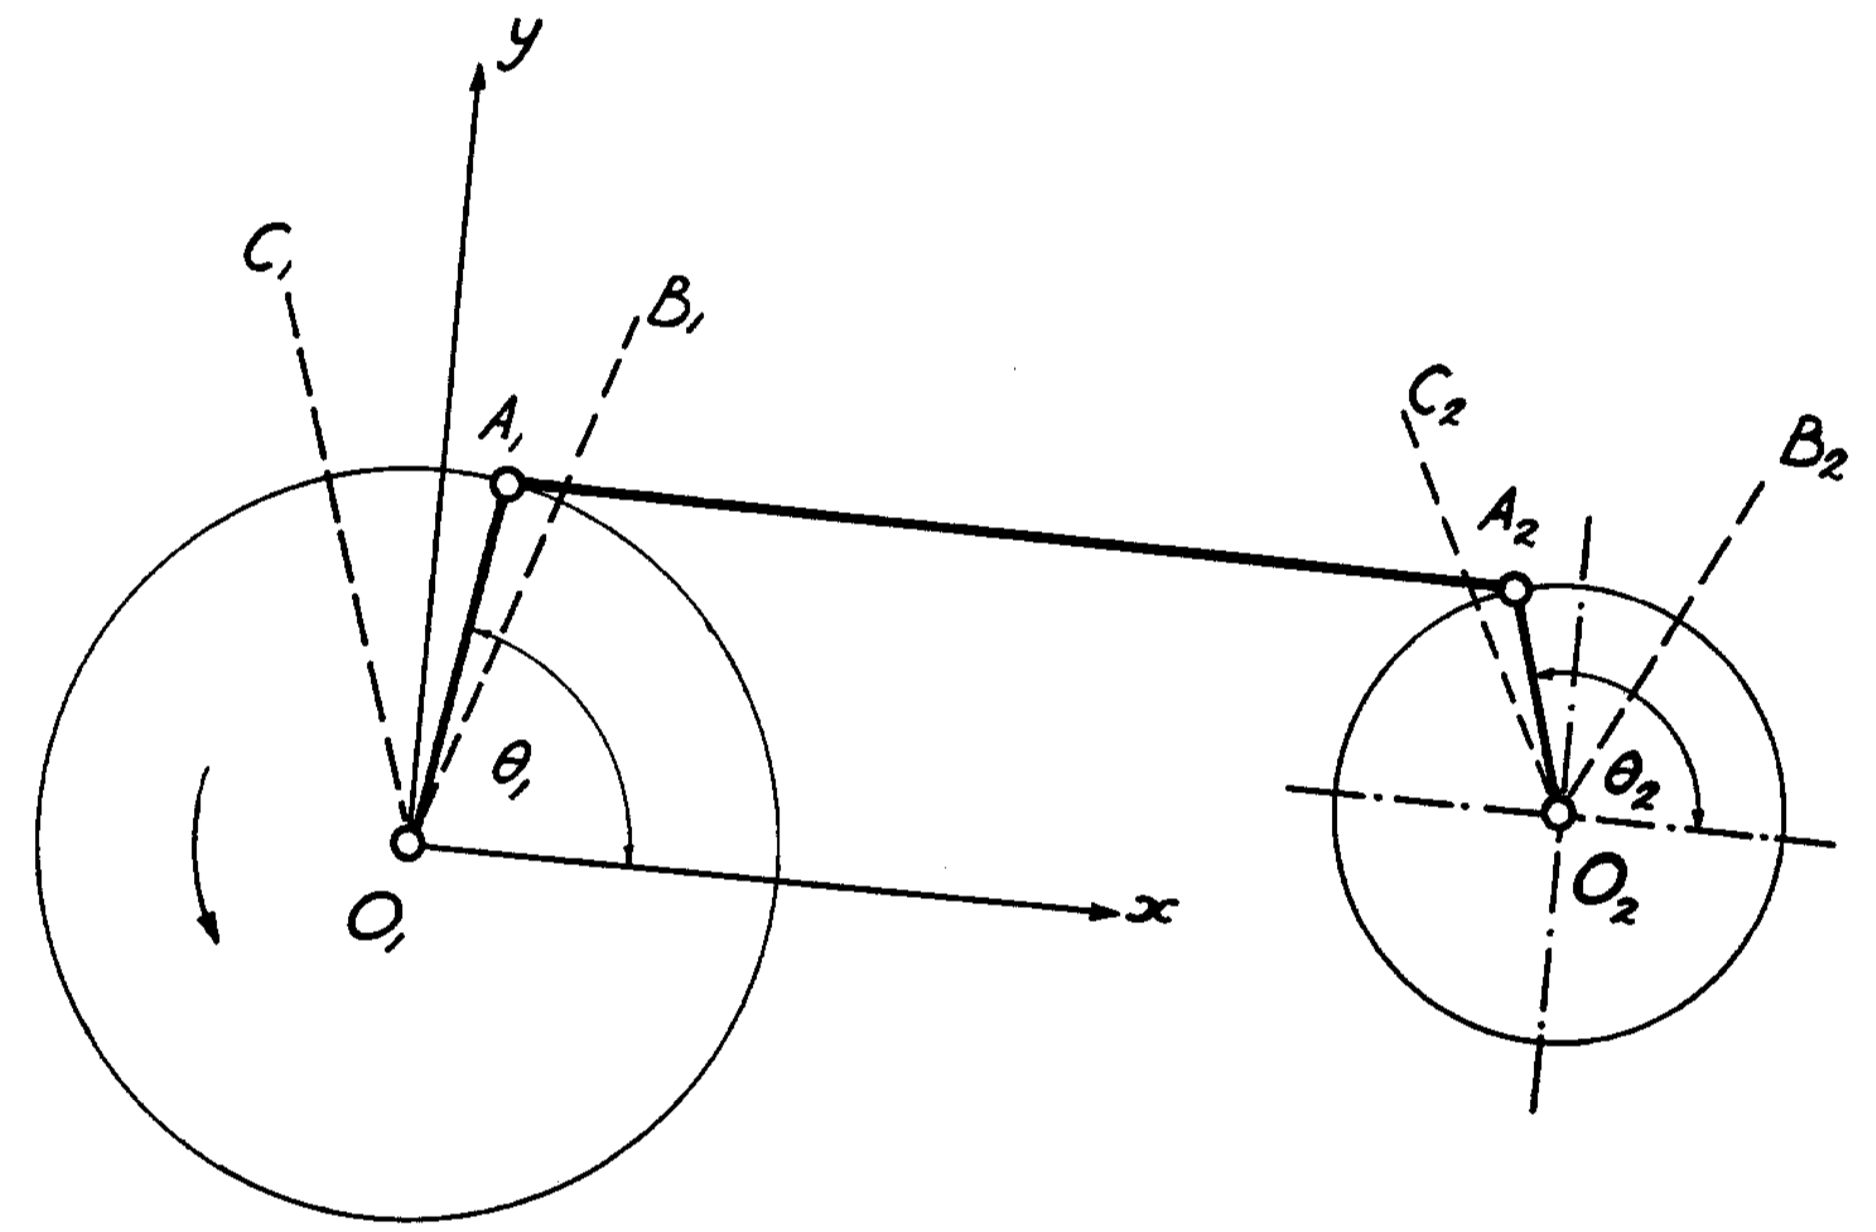
\includegraphics[width=0.9\textwidth]{figs/fig1.png}
  \caption{equivalent four-bar linkage in chain drive}
  \label{fig-poly-1}
\end{figure}

When two equal sprockets are used at a distance apart equal to an integral multiple of the pitch, then $R_1\sin\theta_1$ is always equal to $R_2\sin\theta_2$,and $\dot{\theta}_2$ is constant. In all other cases $\dot{\theta}_2$ will be subject to small fluctuations.

The elasticity of the chain will now be considered. Since each four-bar linkage operates for a period $\tau=\frac{2\pi}{n_1T_1}=\frac{2\pi}{n_2T_2}$ the quantity $R_1\sin\theta_1$ is a function of period $\tau$ and can therefore be expressed as a Fourier series. If we include only the fundamental harmonic term of the series, then it may be shown that

\begin{equation}
  R_1\sin\theta_1 \simeq R_1\frac{T_1}{\pi}\sin\frac{\pi}{T_1}\left[1-\frac{2}{T_1^2-1}\cos pt\right]
  \label{eq-poly-2}
\end{equation}

where $p=n_1T_1=n_2T_2$, and $t$ represents time.

In most power transmitting sprockets the number of teeth is never less than about 15 and therefore the coefficient $\frac{2}{T_1^2-1}$ may be regarded as a small quantity.

Equation~\ref{eq-poly-2} may be written in a simpler form as:

\begin{equation}
  R_1\sin\theta_1 \simeq a_0 + a_1\cos pt
\end{equation}

The speed of $A_1$ is then given by:

\begin{equation}
  -\dot{x}_1 \simeq n_1\left(a_0+ a_1\cos pt\right)
\end{equation}

and by integration:

\begin{equation}
  -x_1 \simeq n_1\left(a_0t+ \frac{a_1}{p}\sin pt\right) + A
  \label{eq-poly-3}
\end{equation}

where $A$ is the constant of integration. In a similar manner it may be shown that:

\begin{equation}
  R_2\sin\theta_2 \simeq Na_0+\frac{a_1}{N}\cos (pt-\alpha)
  \label{eq-poly-4}
\end{equation}

where:

\begin{description}
\item[$\alpha$] a ``phase angle'' corresponding to the fractional pitch in direct common tangent to the pithc circles
\item[$N$] speed ratio $\frac{T_2}{T_1}=\frac{R_2}{R_1}\frac{\frac{T_2}{\pi}\sin\frac{\pi}{T_2}}{\frac{T_1}{\pi}\sin\frac{\pi}{T_1}}$
\end{description}

Equation~\ref{eq-poly-4} has been derived on the assumption that the speed of the driven sprocket is constant. The speed is in fact subject to small fluctuations but it may be shown that the error involved in Equation~\ref{eq-poly-4} is negligible.

Equation~\ref{eq-poly-4} may be written

\begin{equation}
  R_2\sin\theta_2\simeq Na_0+\frac{b_1}{N}\cos pt + \frac{c_1}{N}\sin pt
  \label{eq-poly-5}
\end{equation}

where:

\begin{itemize}
\item $b_1=a_1\cos\alpha$
\item $c_1=a_1\sin\alpha$
\end{itemize}

Let the speed of $A_2$ be given by:

\begin{equation}
  -\dot{x}_2 \simeq \frac{n_1}{N}\left[Na_0+\frac{l_1}{N}\cos pt +\frac{m_1}{N} \sin pt\right]
  \label{eq-poly-6}
\end{equation}

where $l_1$, $m_1$ are constant to be determined.

Integrating and substituting boundary conditions

\begin{equation}
  -\dot{x}_2 \simeq \frac{n_1}{N}\left[Na_0t+\frac{l_1}{pN}\sin pt +\frac{m_1}{pN} \cos pt\right] + A + l
\end{equation}

Now $\dot{\theta}_2 \simeq \frac{-\dot{x}_2}{R_2\sin\theta_2}$ and substituting from \ref{eq-poly-5} and \ref{eq-poly-6} and noting that $b_1$ and $c_1$ are small quantities we get:

\begin{equation}
  \dot{\theta}_2 \simeq \frac{n_1}{N}\left[ 1 + \frac{l_1-b_1}{N^2a_0}\cos pt + \frac{m_1-c_1}{N^2a_0} \sin pt \right]
\end{equation}

This gives

\begin{equation}
  \ddot{\theta}_2 = \frac{N1p}{N^3a_0}\left[(m_1-c_1)\cos pt - (l_1-b_1)\sin pt \right]
\end{equation}

For the oscillation of the driven system about its axis of rotation, the equation of motion is:

\begin{equation}
  I\ddot{\theta}_2 = k(x_1+l-x_2)R_2\sin\theta_2=0
\end{equation}

where $I=$ moment of inertia of driven system about axis of rotation and $k=$ longitudinal stiffness of chain.

Substituting for $\ddot{\theta}_2$, $x_2$, $x_1$ and $R_2\sin\theta_2$ we get

\begin{equation}
  \left[p^2(m_1-c_1)-\omega^2m_1 \right]\cos pt + \left[\omega^2(l_1-a_1N^2)-p^2(l_1-b_1) \right]\sin pt = 0
\end{equation}

where $\omega = \left(\frac{kN^2a_0^2}{I}\right)^\frac{1}{2}$

Since this equation is to be satisfied for all $t$, we get

\begin{equation}
  m_1 = \frac{c_1}{1-\frac{\omega^2}{p^2}}
\end{equation}

and

\begin{equation}
  l_1=\frac{b_1-a_1\frac{N^2\omega^2}{p^2}}{1-\frac{\omega^2}{p^2}}
\end{equation}

\begin{equation}
\text{Dynamic load in chain} =k(x_1+l-x_2)
\end{equation}

\begin{equation}
=\frac{k}{T_1}\left[\left(\frac{l_1}{N^2}-a_1\right)\sin pt - \frac{m_1}{N^2}\cos pt\right]
\end{equation}

Substituting for $l_1$ and $m_1$ the maximum dynamic load is given by

\begin{equation}
  P=\frac{k}{T_1}\left[\left(\frac{b_1}{N^2}-a_1\right)^2+\left(\frac{c_1}{N^2}\right)^2\right]^\frac{1}{2} \frac{1}{1-\frac{\omega^2}{p^2}}
\end{equation}


This shows that the dynamic effect of polygonal action is similar to that of a forced vibration and that large forces may develop when $p$, the circular frequency of tooth engagement, is equal to $\omega$, the natural circular frequency of the system.

Putting

\begin{itemize}
\item $b_1=a_1\cos\alpha$
\item $c_1=a_1\sin\alpha$
\end{itemize}

we get

\begin{equation}
  \begin{split}
  P &\propto \frac{a_1^2}{N^4}\left[\left(\cos\alpha-N^2\right)^2 + \sin^2\alpha\right] \\
  &\propto \frac{a_1^2}{N^4}\left(1-2N^2\cos\alpha+N^4\right)
  \end{split}
\end{equation}

This shows that for a given speed ratio $N$, the dynamic load $P$ is

\begin{itemize}
\item[i] a minimum when $\alpha=0$, that is, integral number of pitches in the direct common tangent.
\item[ii] a maximum when $\alpha=\pi$, that is, an odd number of half pitches in the direct common tangent.
\end{itemize}

As can be expected, the dynamic load is zero when $N = 1$ and $\alpha = 0$, that is, equal sprockets at a distance apart equal to an integral multiple of the pitch.

It is also possible for resonance to occur at half the critical speed, being excited by the second harmonic, but the dynamic load due to this is likely to be small.
